\subsection{Eind punt authenticatie}

Is het proces van een entiteit die zijn identiteit bewijst aan een andere entiteit. Bij het uitvoeren van authenticatie over een netwerk, kunnen de communicerende partijen niet rekenen op biometrische informatie, zoals visuele verschijning of een stem afdruk. Hier moet authenticatie enkel gedaan worden op basis van berichten en data die uitgewisseld worden als een deel van het authenticatie protocol. Normaal wordt die protocol uitgevoerd voordat de twee communicerende partijen andere protocollen gebruiken. Het authenticatie protocol stelt eerst de identiteit van de partijen vast naar elkaars tevredenheid. Enkel na de authenticatie gaan de partijen aan de slag.
We veronderstellen dat Alice zichzelf moet authenticeren aan Bob.

\subsubsection{Authentication Protocol ap1.0}

Het gemakkelijkste AP dat we ons kunnen inbeelden. Alice stuurt een bericht naar Bob waar ze zegt dat ze Alice is.
De fout is duidelijk, er is geen manier voor Bob om te weten wie het bericht stuurt.

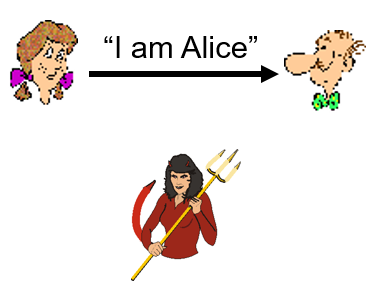
\includegraphics[width=5in]{./img/imghfdst8/hfdst8puntje13.png}\\[1cm]

\subsubsection{Authentication Protocol ap2.0}

Als Alice een bekende netwerk adres heeft vanwaar ze altijd communiceert, kan Bob proberen om Alice te authenticeren door te controleren dat de oorsprong adres op de IP diagram die het authenticatie bericht draagt gelijk is aan Alice’s bekende adres. In dit geval zou Alice geauthenticeerd zijn.
Maar we weten dat het niet zo moeilijk is om een eigen IP diagram te creëren en eender welk bron adres kunnen invoegen. Dit is een vorm van IP spoofing.

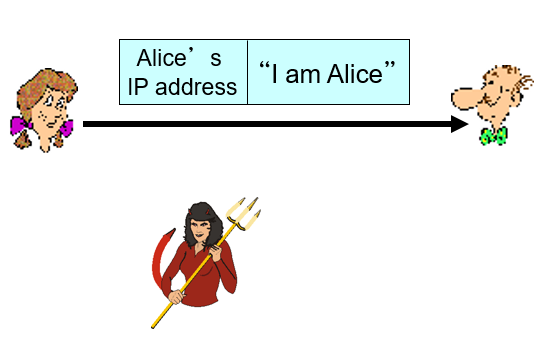
\includegraphics[width=4in]{./img/imghfdst8/hfdst8puntje14.png}\\[1cm]

Mogelijk gevolg: $\rightarrow$ IP-spoofing is mogelijk.

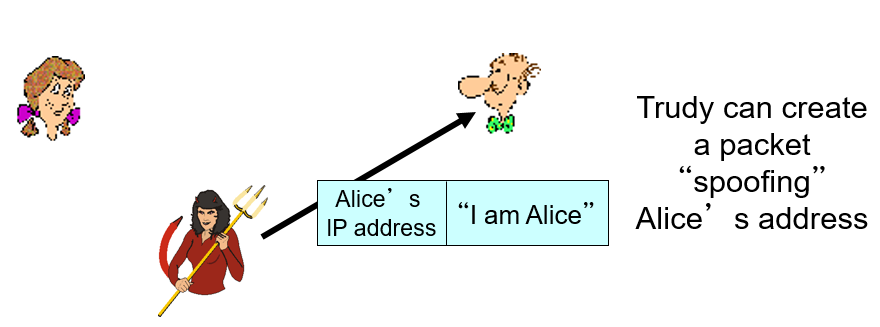
\includegraphics[width=4in]{./img/imghfdst8/hfdst8puntje15.png}\\[1cm]

\subsubsection{Authentication Protocol ap3.0}

Een klassieke benadering is om te authenticeren door middel van een geheim wachtwoord. Het wachtwoord is een gedeeld geheim tussen de authenticator en de person die geauthenticeerd wordt.
Alice zendt dus haar geheim wachtwoord naar Bob. Sinds wachtwoorden zo wijd gebruikt worden, kunnen we vermoeden dat ap3.0 redelijk veilig is.
Maar deze gedacht is fout. Wanneer Trudy meeluistert op Alice’s communicatie, kan ze het wachtwoord van Alice ontrafelen.

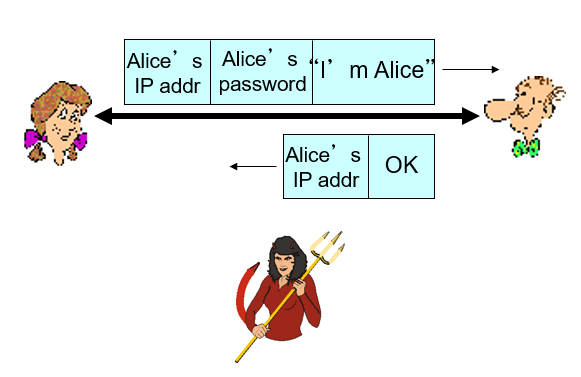
\includegraphics[width=4in]{./img/imghfdst8/hfdst8puntje16.png}\\[1cm]

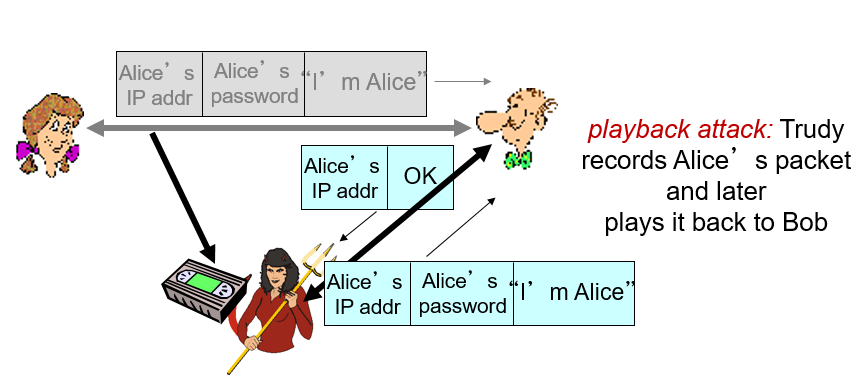
\includegraphics[width=4in]{./img/imghfdst8/hfdst8puntje17.png}\\[1cm]

\clearpage

\subsubsection{Authentication Protocol ap3.1}

Het volgende idee is natuurlijk het wachtwoord encrypteren. Door het wachtwoord te encrypteren kan men voorkomen dat Trudy het wachtwoord te weten komt. We veronderstellen dat Alice en Bob een symmetrische sleutel delen, dan kan Alice haar wachtwoord encrypteren en haar identificatie bericht versturen. Bob decrypteerd het wachtwoord, en veronderstellend dat het wachtwoord correct is, authenticeert Alice. Bob voelt zich comfortabel in het authenticeren van Alice, sinds Alice niet enkel het wachtwoord kent, maar ook de gedeelde geheime sleutel die nodig was om het wachtwoord te encrypteren.
Dit voorkomt dat Trudy het wachtwoord van Alice achterhaalt, maar dit lost het authenticatie probleem niet op. Bob is het onderwerp van een playback attack: Trudy moest enkel Alice’s communicatie afluisteren, de geëncrypteerde versie van het wachtwoord opnemen, en de geëncrypteerde versie van het wachtwoord terug afspelen naar Bob om zich voor te doen als Alice. Dus een geëncrypteerde wachtwoord maakt de situatie niet veel anders.

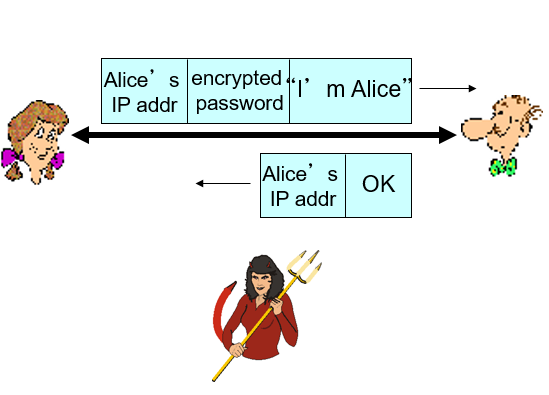
\includegraphics[width=4in]{./img/imghfdst8/hfdst8puntje18.png}\\[1cm]

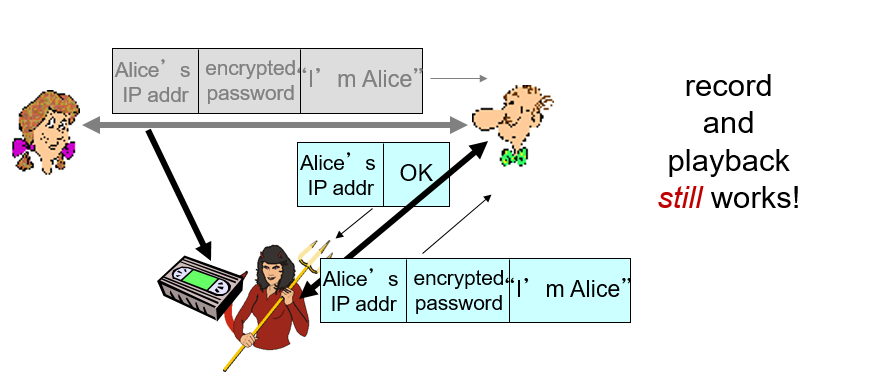
\includegraphics[width=4in]{./img/imghfdst8/hfdst8puntje19.png}\\[1cm]

\subsubsection{Authentication Protocol ap4.0}

In de vorige versie kon Bob niet bepalen of Alice op dit moment wel echt aan de andere kant van de communicatie was of dat de berichten die hij kreeg een opgenomen afspeling van een vorige authenticatie van Alice is. Een nonce is een nummer dat een protocol enkel eenmalig zal gebruiken in zijn bestaan. Wanneer een protocol een nonce heeft gebruikt, dan zal het nummer nooit meer gebruiken. Het protocol gebruikt de nonce als volgt:
\begin{enumerate}
    \item Alice verstuurd een bericht naar Bob.
\item Bob kiest een nonce R, en zend deze naar Alice.
\item Alice encrypteerd de nonce door gebruik te maken de symmetrische sleutel, en verzend de geëncrypteerde nonce terug naar Bob.
\item Bob decrypteerd het ontvangen bericht. Als het gedecrypteerde nonce gelijk is aan de nonce die hij heeft gestuurd naar Alice, dan is Alice geauthentificeerd.

\end{enumerate}

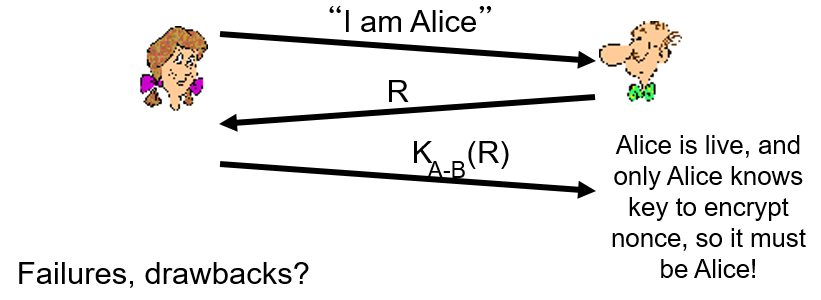
\includegraphics[width=4in]{./img/imghfdst8/hfdst8puntje20.png}\\[1cm]

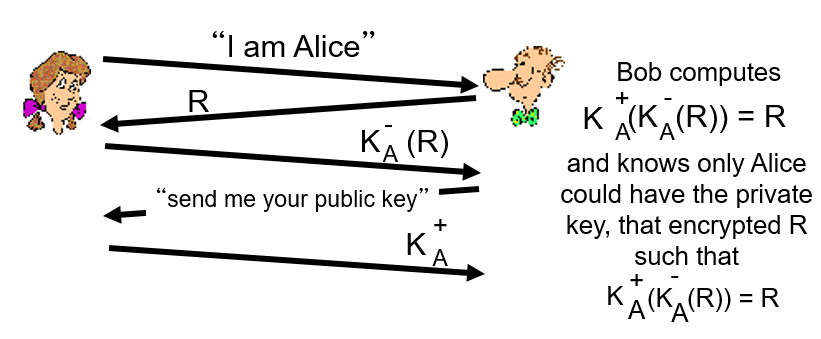
\includegraphics[width=4in]{./img/imghfdst8/hfdst8puntje21.png}\\[1cm]
 

\subsubsection{Authentication Protocol ap5.0}

Er is nog een klein beveiligingsprobleem. Trudy kan zich voordoen als Alice ten opzichte van Bob en als Bob ten opzichte van Alice. Enkel is dit op dit moment moeilijk te achterhalen.

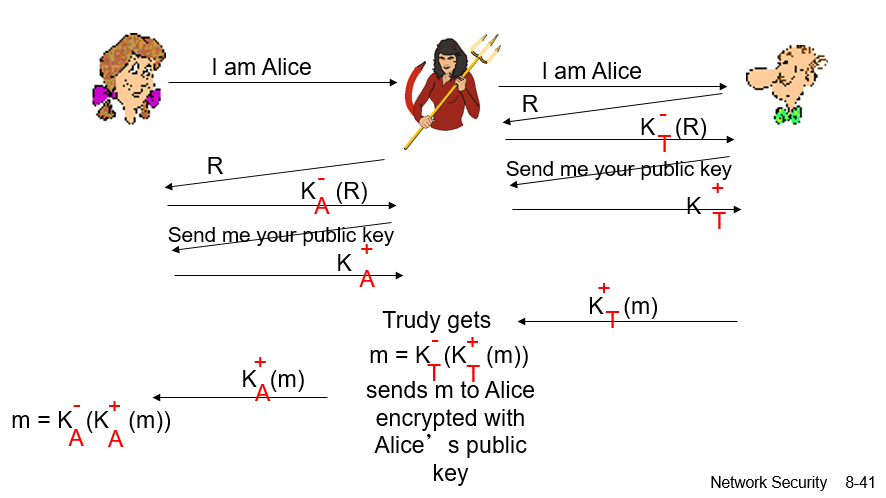
\includegraphics[width=4in]{./img/imghfdst8/hfdst8puntje22.png}\\[1cm]
 